% Standalone RAKL system-architecture diagram (Paper I, Figure 1).
% Build:  pdflatex architecture.tex   -> architecture.pdf
\documentclass[border=6pt]{standalone}
\usepackage{tikz}
\usepackage{helvet}\renewcommand{\familydefault}{\sfdefault}
\usetikzlibrary{positioning,arrows.meta,fit,backgrounds,calc}
\begin{document}
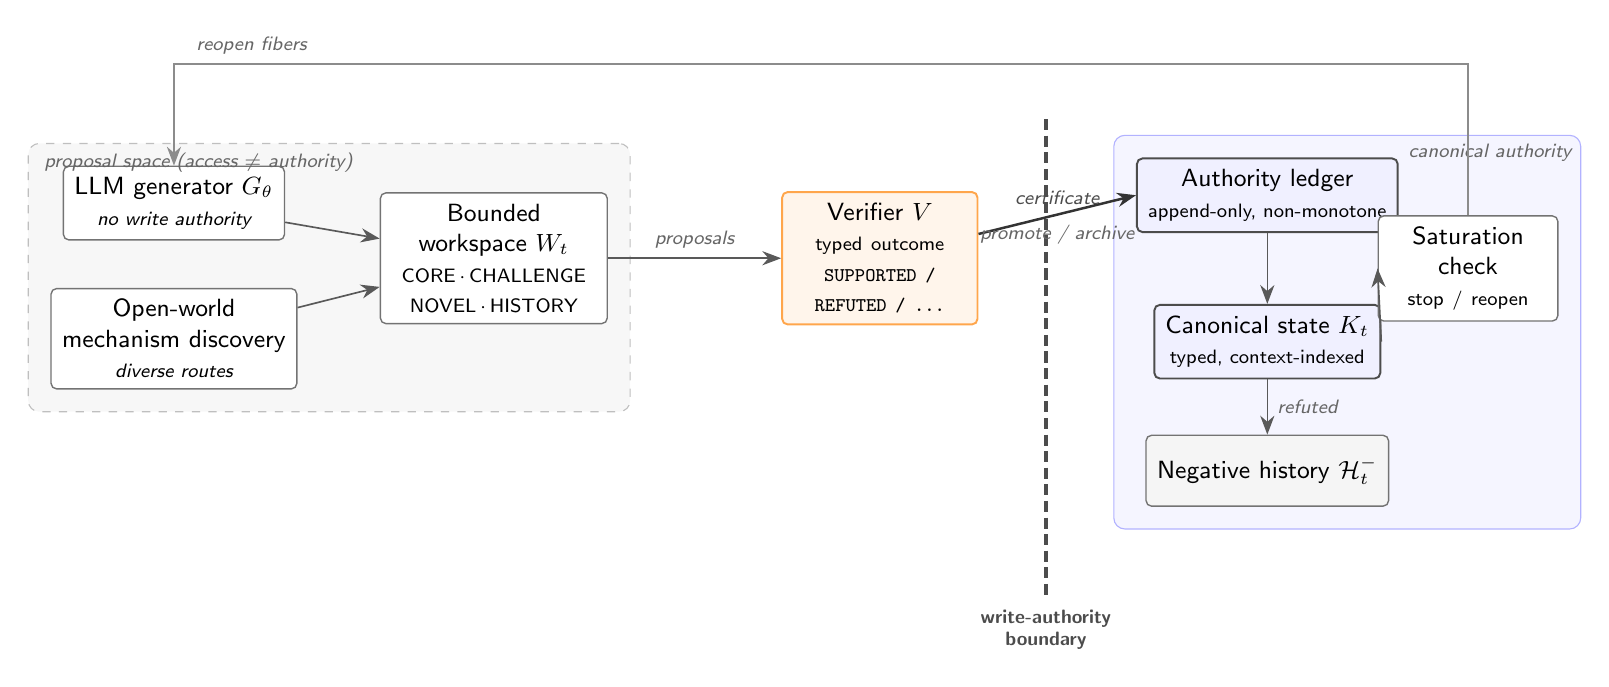
\begin{tikzpicture}[
  font=\small,
  >={Stealth[length=2.4mm]},
  box/.style={rounded corners=2pt, draw=black!55, line width=0.5pt, align=center,
              inner sep=4pt, minimum height=9mm, fill=white},
  store/.style={box, fill=black!4},
  canon/.style={box, draw=black!70, fill=blue!6, line width=0.7pt},
  flow/.style={->, line width=0.6pt, draw=black!65},
  lbl/.style={font=\scriptsize\itshape, text=black!60},
  node distance=6mm and 12mm,
]
% ---- proposal space (left) ----
\node[box] (llm) {LLM generator $G_\theta$\\{\scriptsize\itshape no write authority}};
\node[box, below=of llm] (owmd) {Open-world\\mechanism discovery\\{\scriptsize\itshape diverse routes}};
\node[box, right=of llm, yshift=-7mm, minimum height=15mm, text width=26mm] (ws)
      {Bounded workspace $W_t$\\{\scriptsize CORE\,$\cdot$\,CHALLENGE}\\{\scriptsize NOVEL\,$\cdot$\,HISTORY}};
\begin{scope}[on background layer]
  \node[draw=black!25, dashed, rounded corners=4pt, fill=black!3,
        fit=(llm)(owmd)(ws), inner sep=8pt] (prop) {};
\end{scope}
\node[lbl, anchor=north west] at (prop.north west) {\ proposal space (access $\neq$ authority)};

% ---- verifier on the boundary ----
\node[box, right=22mm of ws, minimum height=15mm, text width=22mm, fill=orange!8, draw=orange!70, line width=0.7pt]
      (ver) {Verifier $V$\\{\scriptsize typed outcome}\\{\scriptsize\ttfamily SUPPORTED /}\\{\scriptsize\ttfamily REFUTED / \dots}};

% ---- canonical authority (right) ----
\node[canon, right=20mm of ver, yshift=8mm] (ledger) {Authority ledger\\{\scriptsize append-only, non-monotone}};
\node[canon, below=9mm of ledger] (state) {Canonical state $K_t$\\{\scriptsize typed, context-indexed}};
\node[store, below=7mm of state] (hist) {Negative history $\mathcal H^-_t$};
\node[box, right=14mm of $(ledger)!0.5!(state)$, text width=20mm] (sat)
      {Saturation\\check\\{\scriptsize stop / reopen}};
\begin{scope}[on background layer]
  \node[draw=blue!30, rounded corners=4pt, fill=blue!4,
        fit=(ledger)(state)(hist)(sat), inner sep=8pt] (canonbox) {};
\end{scope}
\node[lbl, anchor=north east] at (canonbox.north east) {canonical authority\ };

% ---- write-authority boundary (sits in the clear gap between verifier and ledger;
%      only the verified certificate crosses it) ----
\coordinate (bnd) at ($(ver.east)!0.5!(canonbox.west)$);
\draw[line width=1.3pt, black!70, dash pattern=on 4pt off 2pt]
      ($(bnd|-canonbox.north)+(0,2mm)$) -- ($(bnd|-canonbox.south)-(0,9mm)$);
\node[below, font=\scriptsize\bfseries, text=black!70, align=center]
      at ($(bnd|-canonbox.south)-(0,9mm)$) {write-authority\\boundary};

% ---- flows ----
\draw[flow] (llm) -- (ws);
\draw[flow] (owmd) -- (ws);
\draw[flow] (ws) -- node[lbl,above]{proposals} (ver);
\draw[flow, line width=0.9pt, draw=black!80] (ver) -- node[lbl,above,text=black!70]{certificate}
      node[lbl,below]{promote / archive} (ledger.west);
\draw[flow] (ledger) -- (state);
\draw[flow] (state) -- node[lbl,right]{refuted} (hist);
\draw[flow] (state.east) -- (sat.west);
% saturation feedback loop back to proposal space
\draw[flow, draw=black!45] (sat.north) |- ($(prop.north)+(0,10mm)$) -| node[lbl,above,pos=0.25]{reopen fibers} (llm.north);
\end{tikzpicture}
\end{document}
